\documentclass[11pt]{article}
\usepackage{oz,times}

\usepackage{tikz}
\usetikzlibrary{arrows}
\usetikzlibrary{calc}

\title{A Formal Framework for Content-based Retrieval}
\author{Mark d'Inverno and Christophe Rhodes and Michael Jewell}


\begin{document}
\maketitle

%%\begin{gendef}[X]
%%	concat : (\seq (\seq X)) \fun (\seq X)
%%\where 
%%	\forall xs : \seq X; xss : \seq (\seq X) @ \\
%%\t2		concat~ ((\langle xs \rangle) \cat xss) = xs \cat
%%(concat~xss)  
%%\end{gendef}

%% \begin{gendef}[X]
%%	nfront :  \nat \fun (\seq X)  \fun \seq (\seq X) \\
%% \where 
%%	\forall  n : \nat ; xs : \seq X @ \\
%%		n > \# xs \implies nfront ~n~xs = \langle \rangle  \land \\
%%		n \leq \# xs \implies nfront~n~xs =   \\ 
%%		\t2 (\langle 	(0 \upto n-1) \dres xs    \rangle)    \cat (nfront~n~(tail~xs))
%% \end{gendef}

\section{The System Instance}

\newcommand{\LET}{\mathrel{\sf Let}}

\newcommand{\mylet}{\methrel{\sf Let}}
\newcommand{\FV}{\mathrel{~FV}}
\newcommand{\V}{\mathrel{~FV^{d}}}
\newcommand{\U}{\mathrel{~FV^{1}}}
\newcommand{\R}{\mathrel{~R}}

\newcommand{\mylog}{\mathrel{ln}}

\begin{enumerate}

\item \textsf{Track} - original media.

We define the set of all such tracks.

\begin{flushright}
  \begin{tikzpicture}
    \input track.tikz
  \end{tikzpicture}
\end{flushright}

\begin{zed}
[Track]  
\end{zed}

%% \begin{zed}
%%\R == \nat 
%% \end{zed}

%% \begin{axdef}
%% \mylog : \R \fun \R 
%% \end{axdef}

% For every track it is possible to determine the  lenth. 

% \begin{axdef}
%	lenth : Track \fun Time
% \end{axdef} 

% For every track it is possible to determine the  lenth. 

% \begin{axdef}
%	lenth : Track \fun Time
% \end{axdef} 

\item \textsf{Catalogue} - a non-empty list of tracks.

% A catalogue is typically generated for a specific \emph{use case}.  

\begin{flushright}
  \begin{tikzpicture}
    \draw (-3,-3) rectangle (3,3);
    \foreach \y/\xscale in {2/1,1/1.02,0/0.87,-1/0.95} {
      \begin{scope}[yshift=\y cm]
        \begin{scope}[xscale=\xscale]
          \input track.tikz
        \end{scope}
      \end{scope}
    }
    \draw node at (0,-2) {\vdots};
  \end{tikzpicture}
\end{flushright}

\begin{zed}
	Catalogue  == \seq_1 Track 
\end{zed}

\item \textsf{Collection} - a set of catalogues where each track in each catalogue is associated with a unique name.

In a collection, each track has a unique \textsf{TrackName}. We define the injective function $name$ to do this. 

\begin{zed}
	[TrackName]
\end{zed}

\begin{schema}{Collection}
	collection : \power Catalogue 		\\
	tracks : \power Track 			\\
	name : Track \inj TrackName 
\where
	tracks = \{ cat : collection; t : Track | t \in (\ran cat) @ t \}  \\
	\dom name = tracks
\end{schema}

\item \textsf{Time} - the set of non-negative reals. 


\begin{zed}
	Time == \R
\end{zed}


\item \textsf{Interval} - defined as a continuous set of real numbers,  represented as an ordered pair of reals with the second of the pair strictly greater.  

\begin{flushright}
  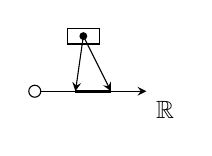
\begin{tikzpicture}[>=stealth]
    \draw (0,0.8) rectangle (0.4,1);
    \fill (0.2,0.9) ellipse (0.05);
    \draw[->] (0.2,0.9) -- (0.1,0.2);
    \draw[->] (0.2,0.9) -- (0.55,0.2);
    \draw[very thick] (0.1,0.2) -- (0.55,0.2);
    \draw[o->] (-0.5,0.2) -- (1,0.2) node[anchor=north west] {\small $\mathbb{R}$};
  \end{tikzpicture}
\end{flushright}

\begin{zed}
	Interval == \{ t_1, t_2 : Time | t_2 > t_1 @ (t_1, t_2) \} 
\end{zed}

\item \textsf{Interval Index} - list of intervals such that the start of each successive interval strictly increases.  Intervals may be overlapping. 

The predicate below states that for any consecutive intervals in an interval index $i_j$ and $i_{j+1}$, that $i_j$ starts before $i_{j+1}$.

\begin{flushright}
  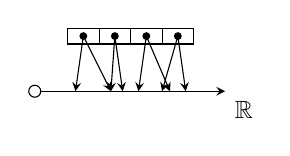
\begin{tikzpicture}[>=stealth]
    \draw (0,0.8) rectangle (1.6,1);
    \draw (0.4,0.8) -- (0.4,1);
    \draw (0.8,0.8) -- (0.8,1);
    \draw (1.2,0.8) -- (1.2,1);
    \fill (0.2,0.9) ellipse (0.05);
    \fill (0.6,0.9) ellipse (0.05);
    \fill (1.0,0.9) ellipse (0.05);
    \fill (1.4,0.9) ellipse (0.05);
    \draw[->] (0.2,0.9) -- (0.1,0.2);
    \draw[->] (0.2,0.9) -- (0.55,0.2);
    \draw[->] (0.6,0.9) -- (0.55,0.2);
    \draw[->] (0.6,0.9) -- (0.7,0.2);
    \draw[->] (1.0,0.9) -- (0.9,0.2);
    \draw[->] (1.0,0.9) -- (1.3,0.2);
    \draw[->] (1.4,0.9) -- (1.2,0.2);
    \draw[->] (1.4,0.9) -- (1.5,0.2);
    \draw[o->] (-0.5,0.2) -- (2,0.2) node[anchor=north west] {\small $\mathbb{R}$};
  \end{tikzpicture}
\end{flushright}

\begin{zed}
	IntervalIndex == \iseq Interval   \\ \\ \\
\end{zed}

\[ 	\forall i : IntervalIndex; i_j, i_{j+1} : Interval @  \\
\t3	\langle i_j, i_{j+1} \rangle \inseq i \implies first~ i_j \leq first ~ i_{j+1}
	\]

\item \textsf{Continuous Interval Index - CII} - there are no consecutive intervals $i_j$ and $i_{j+1}$ in the index where the second element of $i_j$ is strictly less than the first element of $i_{j+1}$.  

\begin{flushright}
  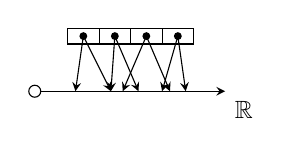
\begin{tikzpicture}[>=stealth]
    \draw (0,0.8) rectangle (1.6,1);
    \draw (0.4,0.8) -- (0.4,1);
    \draw (0.8,0.8) -- (0.8,1);
    \draw (1.2,0.8) -- (1.2,1);
    \fill (0.2,0.9) ellipse (0.05);
    \fill (0.6,0.9) ellipse (0.05);
    \fill (1.0,0.9) ellipse (0.05);
    \fill (1.4,0.9) ellipse (0.05);
    \draw[->] (0.2,0.9) -- (0.1,0.2);
    \draw[->] (0.2,0.9) -- (0.55,0.2);
    \draw[->] (0.6,0.9) -- (0.55,0.2);
    \draw[->] (0.6,0.9) -- (0.9,0.2);
    \draw[->] (1.0,0.9) -- (0.7,0.2);
    \draw[->] (1.0,0.9) -- (1.3,0.2);
    \draw[->] (1.4,0.9) -- (1.2,0.2);
    \draw[->] (1.4,0.9) -- (1.5,0.2);
    \draw[o->] (-0.5,0.2) -- (2,0.2) node[anchor=north west] {\small $\mathbb{R}$};
  \end{tikzpicture}
\end{flushright}

%%unchecked
\begin{zed}
	ContIntIndex == \\
	\t1 \{ ii : IntervalIndex;  i_j, i_{j+1}: Interval  |   \\
 	\t3 \langle i_j, i_{j+1} \rangle \inseq ii \implies  second ~ i_j \geq first ~ i_{j+1}@ ii \}
 \end{zed}

\item \textsf{Standard Interval Index - SII} - a Continual Interval Index which has no overlapping intervals and begins at 0. 

%%unchecked
\begin{zed}
	StandardIntIndex == \\
	\t1 \{ cii : ContIntIndex; i_j, i_{j+1}: Interval | \\
	\t3 first (head~cii) = 0 \land \\
	\t4 second ~ i_j = first ~ i_{j+1}
\end{zed}
% In fact this enables us to specify such a data structure simply as a sequence of increasing times as we can assume the track starts at 0. 

% \begin{zed}
%	ContIntIndex == \iseq Time   \\ \\ \\
% \end{zed}

%% \begin{zed}
%% ContIntIndex == IntervalIndex
%% \end{zed}

\item A \textsf{Duration} is an amount of time. 

\begin{zed}
	Duration == Time
\end{zed}

\item The \textsf{Track Duration} is the duration of a track. It is the difference between the \emph{end} time and \emph{start} time of the track. 

\begin{axdef}
	trackduration : Track \fun Duration 
\end{axdef}

\item \textsf{Interval Duration} is the duration of an interval. It is calculated by subtracting the first element of the interval from the second element. 

\begin{axdef}
	intervalduration : Interval \fun Duration 
\where
	\forall i : Interval @ intervalduration ~ i = second ~ i - first ~ i 
\end{axdef}


\item \textsf{Index Duration} is the duration of a Continuous Interval Index which is simply the second element of the last interval pair. 

\begin{axdef}
	indexduration : ContIntIndex \fun Time 
\where
\forall cii : ContIntIndex @ indexduration~cii = second (last~cii) - first (head~cii)
\end{axdef} 

\item \textsf{Segmenter} - a process which computes an interval index  for any track, represented as a function which maps any track to an interval index.

\begin{flushright}
  \begin{tikzpicture}
    \input interval-index.tikz
    \input segmented-track.tikz
  \end{tikzpicture}
\end{flushright}


In this specification we will consider segmenters that produce a standard interval index. 

\begin{zed}
	Segmenter == Track \fun StandardIntIndex  \\
\end{zed}

\item The \textsf{Length} of an interval index is the number of intervals contained within it. 

\begin{axdef}
	length : IntervalIndex \fun \nat 
\where
	\forall ii : IntervalIndex @ length~ii = \# ii
\end{axdef}

% \section{Features}

\item \textsf{Feature Name} - a name describing a feature.

\begin{zed}
	[FeatureName]
\end{zed}

\item \textsf{Dimension} - a natural number.

\begin{zed}
	Dimension ==	 \nat
\end{zed}

\item \textsf{Feature Kind} - a feature name and associated set of parameters. 

\begin{zed}
	[Const, Var]
\end{zed}

We define the binding type as the set of functions between variables and constants. 

\begin{zed}
	Binding == \power (Var \cross Const) 
\end{zed}

Every feature kind has a dimension (not necessarily fixed). 

\begin{schema}{FeatureKind}
	name :  FeatureName \\
	parameters : \power Var \\
	dparameters : \power Var \\
	binding : Binding \\
	ddimension : Binding \pfun Dimension  \\ 
\where
	dparameters  \subseteq parameters  \\
	\forall b : Binding |  b \in (\dom ddimension) @ dparameters \subseteq  (\dom b) 
\end{schema}

\item A \textsf{Feature} -  sometimes referred to as a Fully Qualified Feature - is  a feature kind with all parameters bound. 

\item \textsf{Feature Dimension} - every feature has a fixed  dimension. 

\begin{schema}{Feature}
	FeatureKind \\
	fdimension : Dimension  \\
\where
	\dom binding = parameters \\
	fdimension = ddimension~binding
\end{schema}

\item \textsf{Unit Feature} - any feature with a dimension of 1.
	
\begin{schema}{UnitFeature}
	Feature \\
\where
	fdimension = 1
\end{schema}

\item \textsf{Feature Vector} - a non-empty sequence of real numbers.

\begin{zed}
	\FV == \seq_1 \R 
\end{zed}

% DEFINE ALL FEATURE VECTORS HERE 

%% \begin{zed}	
%% \V == \FV \\
%% \U  == \FV 
%% \end{zed}

\newcommand{\Vdsl}{\mathrel{~FV^{d * sl}}}

%% \begin{zed}
%% \Vdsl == \FV
%% \end{zed}

\newcommand{\Vd}{\mathrel{~FV^{d}}}

%% \begin{zed}
%% \Vd == \FV
%% \end{zed}

\newcommand{\Z}{\mathrel{~FV^{1}}}

%% \begin{zed}
%% \Z == \FV
%% \end{zed}

\newcommand{\Vsl}{\mathrel{~FV^{sl}}}

%% \begin{zed}
%% \Vsl == \FV
%% \end{zed}


\item \textsf{Feature Vector Dimension} - the length of a feature vector. 

\begin{axdef}
	dimension : \FV \fun \nat
\where
	\forall fv : \FV @ dimension~fv = \# fv
\end{axdef}

\item \textsf{Unit Vector} - any feature vector with a dimension of 1.

\begin{zed}
	UnitVector == \{ fv : \FV | dimension~fv = 1 \}
\end{zed}

\item \textsf{Extractor} - a  process which computes a feature vector of fixed dimension for any interval of any track, represented formally as a function that takes a track and an interval and returns a feature vector.

\begin{zed}
	Extractor ==  Track \fun Interval \fun \FV 
\end{zed}

\item \textsf{Unit Extractor} - a subclass of Extractor where the feature vector dimension is equal to 1.

\begin{zed}
	UnitExtractor ==  \\
\t1		\{ e : Extractor | \forall t : Track; i : Interval @ dimension (e~t~i) = 1 \}  
\end{zed}

\item \textsf{Bel Unit Extractor} - a subclass of Unit Extractor where the function outputs on the bel scale (between minus infinity and zero). 

\begin{zed}
	BelUnitExtractor ==  UnitExtractor
\end{zed}

The range of the real contained in the bel unit vector is less than 0. 

\begin{zed}
		\forall t : Track; int : Interval; ux : BelUnitExtractor   @  \\
		\t5 head (ux~t~int)  \leq 0
\end{zed}


\item \textsf{Feature Extractors} - the set of  all extractors associated with a feature.

As this data structure can be updated over time -  by adding and removing new features, and adding and removing extractors for a feature as new ones arise and old ones are not used - we use a schema. The  predicate states that the feature vector dimension computed by an extractor must be equal to the associated feature dimension. Every feature has a unique associated unit feature  and every extractor has a unique associated unit extractor. Once a user defines a feature, and one its associated extractors, the unit feature and extractor are generated automatically.  

\begin{schema}{FeatureExtractors}
	featureextractors : Feature \pfun (\power Extractor) \\
	features : \power Feature \\
	extractors : \power Extractor \\
\where
	\dom featureextractors = features \\
	\bigcup (\ran featureextractors) = extractors \\
	\forall f : Feature ; e :  Extractor ; t : Track; i : Interval \\
	\t1 @ e \in featureextractors(f)  \implies  \\
	\t2 f.fdimension = dimension (e~ t ~ i) \\
\end{schema}

\item \textsf{Track Feature Vectors} - given a segmenter and an extractor the  sequence of feature vectors  for each interval of the track 

\begin{flushright}
  \begin{tikzpicture}
    \input track-feature-vectors.tikz
  \end{tikzpicture}
\end{flushright}

The function $extract$ applies an extractor to each interval of a track to return a list of feature vectors. This  requires  the generic function  map, which takes a function and applies it to every element of a list. A definition can be found in the appendix. 

%%\begin{gendef}[X,Y]
%%	map : (X \fun Y) \fun (\seq X) \fun (\seq Y) \\
%%\where 
%%	\forall  f : X \fun Y; x : X; xs,ys : \seq X @ \\
%%\t1		map~f~\langle \rangle = \langle \rangle \land \\
%%\t1 		map~f~(xs \cat ys) = map~f~xs \cat map~f~ys 
%%\end{gendef}

\begin{axdef}
extract : Segmenter \fun Extractor \fun Track \fun \seq \FV
\where
\forall seg : Segmenter; fx : Extractor; t : Track @ \\
\t5  extract~seg~fx~t = map ~ (fx~t) (seg~t)
\end{axdef}  


\item \textsf{Track Unit Vectors} - defined as above but specifically for unit extractors

\begin{flushright}
  \begin{tikzpicture}
    \input interval-index.tikz
    \input segmented-track.tikz
%    \foreach \x in {-2.5,-2,-1.4,-0.5,0,0.8,1.3,1.8} {
%      \begin{scope}[xshift=\x cm,yshift=-0.4 cm]
    \foreach \x in {-1.8,-1.4,...,1.1} {
      \begin{scope}[xshift=\x cm,yshift=1.1 cm]
        \draw (-0.1,0) rectangle (0.1,0.2);
      \end{scope}
    }
    \begin{scope}[yshift=1.1 cm]
      \draw[|-|,>=stealth] (-2.3,0) -- (-2.3,0.2);
      \draw node[anchor=south east] at (-2.4,0.1) {\small $d=1$};
    \end{scope}
  \end{tikzpicture}
\end{flushright}

\item \textsf{Catalogue Feature Vectors}  - a sequence of track feature vectors for each track in the catalogue ($features$)

\item  \textsf{Catalogue Unit Vectors}  - a sequence of track unit vectors for each track in the catalogue ($unitfeatures$)

\item \textsf{Catalogue Index} - a sequence of continuous interval indexes (one for each track).

An example can be seen below

\[ \langle 
\langle (0,r_{11}), (r_{11},r_{12}), (r_{12}, r_{13}) \rangle, \\ 
\langle (0,r_{21}), (r_{21},r_{22}), (r_{22}, r_{23}, (r_{23}, r_{24}) \rangle, \\ 
\langle (0,r_{31}), (r_{31},r_{32}), (r_{32}, r_{33}) \rangle, \\
\rangle \]

\item \textsf{Instance} - a catalogue, segmenter, feature, extractor, unit  feature, unit extractor, dimension, feature vectors, catal

% \emph{In our usage (see \textsf{Absolute} \and \textsf{Relative} in section \ref{s:refining}), we require certain semantics of the \textsf{Unit Feature} (and so of the values returned by its \textit{Unit Extractors}.  Specifically, the values returned must be interpretable on a logarithmic scale in Bels, with the maximum possible value being the reference threshold at 0B.}

\begin{schema}{Instance} 
	cat : Catalogue 				\\
%	tracks : \power Track 	\\
	seg : Segmenter  			\\ 
	f : Feature 				\\  
	x : Extractor				\\			
	uf : UnitFeature			\\
	ux : UnitExtractor			\\
	d : Dimension 				\\
	index : \seq ContIntIndex \\
	features  :  \seq ~ (	\seq 	\V) \\
	unitfeatures : \seq ~ (\seq 	\U)  \\
\where
	d = f.fdimension \\
	index = map~seg~cat \\
	features = map ~ (extract~seg~x) ~ cat \\  
	unitfeatures =  map ~ (extract~seg~ux) ~ cat  \\     
\end{schema}	

\item  \textsf{Singleton Instances}  - the set of System instances which contain only one track

\begin{schema}{SingletonInstance} 
	Instance \\
\where
	\# cat = 1 
\end{schema}

\item  \textsf{System Instances}  - the set of system instances.

Note that every instance must contain a catalogue in the music collection but not all catalogues in the collection are necessarily part of an instance. 

\begin{schema}{SystemInstances}
		Collection \\
		instances : \power Instance
\where
		\{ i : instances @ i.cat \} \subseteq collection
\end{schema}
		
\section{Search Vectors}
Searching takes place using concatenations of feature vectors to build \emph{search} vectors. For a particular query all search vectors will have a fixed length equal to some multiple (which we will refer to as $sl$, the search length) of the dimension of the orignal feature vectors ($d$). 

In the schema below, the function $makesearchvs$ takes a natual number $sl$ and a sequence of feature vectors (associated with a track) to create a sequence of search vectors. The first element of the returned sequence is the concatenation of the first $sl$ feature vectors, the second element is also the concatenation the next $sl$ feature vectors but starting from the second element, and so on until all such sequences are formed.  It should be clear that if the original sequence contains $n$ feature vectors then the output will contain $n-sl+1$ vectors. 

\begin{flushright}
  \begin{tikzpicture}[>=stealth]
    \begin{scope}[xshift=-6 cm]
      \input track-feature-vectors.tikz
      \begin{scope}[yshift=1.1 cm]
        \begin{scope}[yshift=1.1 cm,xshift=-1.8cm]
          \input fv1.tikz
          \draw (-0.1,0) rectangle (0.1,1);
          \draw (-0.1,0.2) -- (0.1,0.2);
          \draw (-0.1,0.4) -- (0.1,0.4);
          \draw (-0.1,0.6) -- (0.1,0.6);
          \draw (-0.1,0.8) -- (0.1,0.8);
        \end{scope}
        \begin{scope}[yshift=2.2 cm,xshift=-1.8cm]
          \input fv2.tikz
          \draw (-0.1,0) rectangle (0.1,1);
          \draw (-0.1,0.2) -- (0.1,0.2);
          \draw (-0.1,0.4) -- (0.1,0.4);
          \draw (-0.1,0.6) -- (0.1,0.6);
          \draw (-0.1,0.8) -- (0.1,0.8);
        \end{scope}
        \draw[->] (-1.4,1) arc(0:90:0.4 and 0.6);
        \draw[->] (-1.0,1) arc(0:90:0.8 and 1.7);
        \draw[->] (-1.0,1) arc(0:90:0.4 and 0.6);
        \draw[->] (-0.6,1) arc(0:90:0.8 and 1.7);
      \end{scope}
    \end{scope}
    \input interval-index.tikz
    \input segmented-track.tikz
%    \foreach \x in {-2.5,-2,-1.4,-0.5,0,0.8,1.3,1.8} {
%      \begin{scope}[xshift=\x cm,yshift=-0.4 cm]
    \foreach \x/\f in {-1.8/fv0,-1.4/fv1,-1.0/fv2,-0.6/fv3,-0.2/fv4,0.2/fv5,0.6/fv6,1.0/fv7} {
      \begin{scope}[yshift=1.1 cm,xshift=\x cm]
        \input \f.tikz
      \end{scope}
    }
    \foreach \x/\f in {-1.8/fv1,-1.4/fv2,-1.0/fv3,-0.6/fv4,-0.2/fv5,0.2/fv6,0.6/fv7} {
      \begin{scope}[yshift=2.1 cm,xshift=\x cm]
        \input \f.tikz
      \end{scope}
    }
    \foreach \x/\f in {-1.8/fv2,-1.4/fv3,-1.0/fv4,-0.6/fv5,-0.2/fv6,0.2/fv7} {
      \begin{scope}[yshift=3.1 cm,xshift=\x cm]
        \input \f.tikz
      \end{scope}
    }
    \foreach \x in {-1.8,-1.4,...,0.3} {
      \begin{scope}[xshift=\x cm,yshift=1.1 cm]
        \draw (-0.1,0) rectangle (0.1,3);
        \foreach \y in {0.2,0.4,...,2.9} {
          \draw (-0.1,\y) -- (0.1,\y);
        }
      \end{scope}
    }
    \begin{scope}[yshift=1.1 cm]
      \draw[<->,>=stealth] (-2.1,0) -- (-2.1,3);
      \draw node[anchor=east] at (-2.3,1.5) {$d \times sl$};
    \end{scope}
    \begin{scope}[yshift=1.1 cm]
      \draw[<->,>=stealth] (-2,3.2) -- (0.4,3.2);
      \draw node at (-0.8,3.6) {$n - sl + 1$};
    \end{scope}
    \begin{scope}[xshift=0.6 cm,yshift=1.1 cm]
      \draw (-0.1,0) rectangle (0.1,2);
      \foreach \y in {0.2,0.4,...,1.9} {
        \draw (-0.1,\y) -- (0.1,\y);
      }
      \draw[dashed] (-0.1,0) -- (-0.3,1);
      \draw[dashed] (-0.1,1) -- (-0.3,2);
      \draw[dashed] (-0.1,2) -- (-0.3,3);
    \end{scope}
    \begin{scope}[xshift=1.0 cm,yshift=1.1 cm]
      \draw (-0.1,0) rectangle (0.1,1);
      \foreach \y in {0.2,0.4,...,0.9} {
        \draw (-0.1,\y) -- (0.1,\y);
      }
      \draw[dashed] (-0.1,0) -- (-0.3,1);
      \draw[dashed] (-0.1,1) -- (-0.3,2);
    \end{scope}
    \foreach \x in {-1.4,-1.0,...,0.3} {
      \begin{scope}[xshift=\x cm,yshift=1.1 cm]
        \draw[dashed] (-0.1,0) -- (-0.3,1);
        \draw[dashed] (-0.1,1) -- (-0.3,2);
        \draw[dashed] (-0.1,2) -- (-0.3,3);
      \end{scope}
    }
  \end{tikzpicture}
\end{flushright}

\begin{axdef}
 	makesearchvs : \nat \fun  \seq \Vd \fun \seq \Vdsl
\where 
	\forall xs :  \seq \FV ; sl : \nat   @ \\
\t1 sl > \# xs \implies makesearchvs~sl~xs = \langle \rangle  \land \\
\t1 sl \leq \# xs \implies makesearchvs~sl~xs = \\
\t2 concat (\langle (1 \upto sl) \dres xs  \rangle)  \cat  makesearchvs~sl (tail~xs)
\end{axdef}


\item \textsf{Instance Search Vectors}

For any natural number less than the length of feature vectors for each track we can calculate the search vectors for an given by applying the $makesearchvs$ function to each of the sequences of feature vectors.  We call this natural number \emph{search length} ($sl$) and we can use $map$ to apply $makesearchvs ~ sl$ to each of these sequences.  

\begin{schema}{SearchVectors}
	i? : Instance \\
	sl? : \nat \\
	searchvs! :  \seq (\seq \Vdsl) \\  
	unitvs! :  \seq (\seq \Vsl) \\  
\where
	searchvs! =   map ~ (makesearchvs ~ sl?) ~ i?.features  \\
	unitvs! =  map ~ (makesearchvs ~ sl?) ~ i?.unit  \\
\end{schema}

\item \textsf{Hopped Search Vectors}

Rather then generating all possible search vectors we may wish to general vectors starting at equally distanced intervals in the interval index of the tracks in an instance.  We refer to the size of this interval as $hop$. 

\begin{gendef}[X]
    strip : \nat \fun (\seq X) \fun \seq X
    \where
        \forall x : X; xs : \seq X @ \\
	\t1         strip ~ 0  ~ xs = xs \land \\
	\t1        strip ~ (n+1) ~ \langle \rangle = \langle \rangle \\
	\t1         strip ~ (n+1) ~ \langle x \rangle \cat xs = strip ~ n ~ xs
\end{gendef} 

\begin{axdef}
 	makehopsearchvs : \nat \fun  \nat \fun \seq \Vd \fun \seq \Vdsl
\where 
	\forall xs :  \seq \FV ; sl : \nat  ; hop  : \nat  @ \\
\t1 sl > \# xs \implies makehopsearchvs~sl~hop~xs = \langle \rangle  \land \\
\t1 sl \leq \# xs \implies makehopsearchvs~sl~hop~xs = \\
\t2 concat (\langle (1 \upto sl) \dres xs  \rangle)  \cat  \\
\t2 			makehopsearchvs~sl~hop~ (strip~hop~xs)
\end{axdef}

This enables us to define a hop size when generating search vectors

\begin{schema}{HopSearchVectors}
	SearchVectors \\
	hop? : \nat \\
	hopsearchvs! :  \seq (\seq \Vdsl) \\  
	hopunitvs! :  \seq (\seq \Vsl) \\  
\where
	hopsearchvs! =  map ~ (makehopsearchvs ~i?.d ~ hop?) ~ i?.features  \\
	hopunitvs! =  map ~ (makehopsearchvs ~ i?.d ~ hop?) ~ i?.unit  \\
\end{schema}

\item \textsf{Search Vector Power}

For each Search Vector in an instance's search vectors we take the associated unit values and take the arithmetic mean. 

\begin{axdef}
	average : \V \fun \R
\end{axdef}

\begin{schema}{Powers}
	SearchVectors \\
	powers : \seq (\seq \R) 
\where 
	powers = map~(map ~ average) ~  unitvs! \\
\end{schema}

\item \textsf{Search Vector Duration}

The duration of the sequence of the original feature vectors from which the search vector is composed. 

\begin{enumerate}

\item \textsf{Single Search Vector Duration}

This is defined as the duration of the sequence for each search vector. So for example if a search vector was made from the combination of 3 feature vectors and those 3 feature vectors came from the following intervals $ (3,8), (8,11), (11,13) $ then the duration of the search vector is $13-3=10$. 

\item \textsf{Track Search Vector Durations}

Next we define a function at the level of track search vectors. We define a function which takes a sequence of search vectors for that track, the search length that was used to create them, and the track interval index and returns a sequence of natural numbers each of which is the duration of the corresponding search vector

\begin{axdef}
	durationsTsv : \seq \Vdsl  \fun  ContIntIndex \fun \nat \fun  \seq \R
\where
	\forall svs : \seq \Vdsl;  cii :  ContIntIndex; sl : \nat @ \\
	\t1 durationsTsv~svs~cii~sl = \\
	\t2 \{ n : \nat | n \in 1 \upto n - sl + 1 @ \\
	\t3 (n,  first (cii (n + sl)) - first (cii (n)) ) \} 
\end{axdef}

\item \textsf{Instance Search Vector Durations}

Finally, we define a function called svdurations which takes a sequence of search vectors and calculates the track search vector durations for each sequence.

\begin{axdef}
	durationsIsv : \seq (\seq \Vdsl) \fun (\seq ContIntIndex) \fun \nat \fun  \seq (\seq \R) \\
\where
	\forall svss : \seq (\seq \Vdsl); sl : \nat; ciis :  \seq ContIntIndex @ \\
\t1 	 	durationsIsv ~ svss ~ ciis ~ sl =  \\
\t2		\langle durationsTsv  ~ (head ~ svss) ~ (head ~ ciis) ~ sl   \rangle  \cat \\
\t3  durationsIsv ~ (tail ~ svss) ~ (tail ~ ciis) ~ sl  \land \\
\t1		durationsIsv ~ \langle \rangle~ \langle \rangle ~ sl = \langle \rangle 
\end{axdef}

\end{enumerate}

\begin{schema}{Durations}
	SearchVectors \\
	svdurations! : \seq (\seq \R) \\	
\where
	svdurations! = durationsIsv ~ searchvs! ~ i?.index ~ sl? 
\end{schema}

% \end{enumerate}

\section{Making a Query}

\item \textsf{General Instance Query}

Two instances, a source and a target are identified by the user for comparison as well as the search length from which the search vectors are defined for both the source and the sequence.  Once the query has been defined we can generate the \emph{source search vectors},  \emph{source unit vectors},   \emph{target search vectors} and \emph{target unit vectors} as specified earlier. We also generate \emph{source powers}, \emph{target powers}, \emph{source search vector durations} and \emph{target search vector durations}. 

\emph{What are the pre-conditions regarding the search length? That it is less than the length of any sequence of feature vectors for every track?}

\begin{schema}{GeneralQuery}
	SystemInstances \\
	src?, tgt? : Instance  \\
	sl?: \nat \\
	srcsearchvs!,   tgtsearchvs! :  \seq (\seq \Vdsl) \\  
	srcunitvs!,  tgtunitvs! :  \seq (\seq \Vsl) \\  
	sourcepowers, targetpowers : \seq (\seq \R) \\
	sourcedurations, targetdurations :  \seq (\seq \R) \\
\where
	\{ src?, tgt? \} \subseteq instances \\
\end{schema}
	
\item \textsf{General Instance Self Query}

When an instance is identified as both the source and target we state that it is a self query. 

\begin{schema}{GeneralSelfQuery}
	GeneralQuery
\where
	src? = tgt?
\end{schema}

\item Singleton  (Track)  Query

A user defines an instance with exactly one track as the source. 

\begin{schema}{SingletonQuery}
	GeneralQuery
\where
	src? \in SingletonInstance
\end{schema}
  
\item Point (Sequence) Query

The user identifies a specific part of the track in a singleton instance to be used as the source known as a \emph{sequence}.  A user defines the sequence by  specifying the start and end points of the sequence index. Once these have been defined the sequence, sequence index and sequence length are easily identified. 

\begin{enumerate}

\item \textsf{Source track} - the single track contained in the instance. 

\item \textsf{Sequence} - a continuous sub-section of the point query track used to make a	 query. 

\begin{zed}
	Sequence == Track
\end{zed}

\item \textsf{Sequence Index} - a continuous interval index that defines the sequence according to the segmenter of the instance. 

% \emph{Can we discuss this - is it reset so that the first element is indexed by 1 and so on?}

\item \textsf{Sequence Length} - the number of  intervals in the sequence index.

\end{enumerate}

\begin{schema}{PointQuery}
	GeneralQuery \\
	start?, end? :  \nat \\
	sourcetrack? : Track \\
	sequence! : Sequence \\
      	seqindex! : ContIntIndex \\
	sl! : \nat \\
\where
	sourcetrack? \in \ran cat \\
	start? \in \dom (src?.seg (sourcetrack?)) \\ 
	end? \in \dom (src?.seg (sourcetrack?)) \\ 
	seqindex! =  (start? \upto end?) \dres (src?.seg~sourcetrack?)   \\
	sl! = end? - start? \\
\end{schema}

In this case the search vectors will be equal to a sequence containing only one sequence. That sequence will be a search vector of dimension $d * sl$ where $d$ is the dimension of the sequence and $sl$ the length of the sequence. 

\[  \langle \langle \Vdsl \rangle \rangle \]

\section{Distance between Search Vectors}	

We define the scalar product and distance between vectors of equal dimension. 

\begin{axdef}
	scalarproduct : \V \fun \V \fun \R \\
	distance : \V \fun \V \fun \R \\
\end{axdef}

\begin{zed}
	\forall v_1, v_2 : \V @  distance~v_1~v_2 = 2 - scalarproduct~v_1~v_2		
\end{zed}

Then we can define a variable which maintains a list of all distances between the  source and target search vectors. If we have a sequence of sequence of search vectors in the both the source and the target we will end up with a sequence of sequence of sequence of sequences. 

For the purposes of illumination imagine a source and target each with two simple search vectors. Again, we will replace the reals with naturals here. 

Let us assume we have the following source search vectors for an instance of two tracks

\[ \langle \langle  a_1, a_2, a_3  \rangle, \langle b_1, b_2 \rangle \rangle \]

And the following target search vectors also for an instance of two tracks

\[ \langle \langle  x_1, x_2   \rangle, \langle y_1, y_2, y_3 \rangle \rangle \]
     
Then we need to generate the following data structure 

\[   \langle 		\\ % First track in source with  target instance   \\
 \t1              \langle   \\ % First Search Vector with whole of target \\
	\t2			\langle 	 \\ % First Search Vector with first track
		\t3			     \langle  a_1 \dot x_1, a_1 \dot x_2 \rangle,   \\
		\t3			     \langle  a_1 \dot y_1, a_1 \dot y_2, a_1 \dot y_3 \rangle \\
	\t2	              \rangle,   \\
		              % Second search vector 
	\t2	              \langle \\
		\t3              	     \langle  a_2 \dot x_1, a_2 \dot x_2 \rangle,   \\
		\t3			     \langle  a_2 \dot y_1, a_2 \dot y_2, a_2 \dot y_3 \rangle \\
	\t2	              \rangle, \\
	\t2	               \langle \\
		\t3              	     	     \langle  a_3 \dot x_1, a_3 \dot x_2 \rangle,   \\
		\t3			     \langle  a_3 \dot y_1, a_3 \dot y_2, a_3 \dot y_3 \rangle  \\
	\t2	              \rangle  \\
\t1		  \rangle,  \\
		  % Second track in source with  target instance
\t1		  \langle,             \\
	\t2	              \langle  \\
		\t3			     \langle  b_1 \dot x_1, b_1 \dot x_2 \rangle,  \\
		\t3			     \langle  b_1 \dot y_1, b_1 \dot y_2, b_1 \dot y_3 \rangle   \\
	\t2	              \rangle   \\
	\t2	              \langle    \\
		       \t3       	            \langle  b_2 \dot x_1, b_2 \dot x_2 \rangle,    \\
			\t3		     \langle  b_2 \dot y_1, b_2 \dot y_2, b_2 \dot y_3 \rangle   \\
	\t2	              \rangle		 \\
   \t1           \rangle  \\
       \rangle        \\
 \]
		            

First let us define the function to calculate the distances for a single search vector.

\begin{axdef}		
	vectordistances : \Vdsl \fun \seq (\seq \Vdsl) \fun \seq (\seq \R) 
\where
	\forall sv : \Vdsl; targetsv : \seq (\seq \Vdsl) @ \\
	\t1  vectordistances~sv~targetsv = map (map (distance~sv)) targetsv
\end{axdef}

Next we define the function for calculating the distances for the search vectors of a track with a target instance. 

\begin{axdef}		
	trackdistances : (\seq \Vdsl) \fun \seq (\seq \Vdsl) \fun \seq (\seq (\seq \R)) 
\where
	\forall tracksv : \seq \Vdsl; targetsv : \seq (\seq \Vdsl) @ \\
	\t1  trackdistances~tracksv~targetsv = \\
	\t3 \langle vectordistances~(head ~ tracksv)~targetsv \rangle \cat \\
     \t4										  trackdistances~(tail ~ tracksv) ~ targetsv \land \\
     \t1  trackdistances~\langle \rangle ~targetsv = \langle \langle \langle \rangle \rangle \rangle 
\end{axdef} 
     
Then we can define a function which calculating the distances between a source and target instance. 

\begin{axdef}		
	instancedistances : \seq (\seq \Vdsl) \fun \seq (\seq \Vdsl) \fun \seq (\seq (\seq (\seq \R)))
\where
	\forall sourcesv, targetsv: \seq (\seq \Vdsl) @ \\
	\t1  instancedistances~sourcesv~targetsv = \\
	\t3 \langle trackdistances~(head ~ sourcesv)~targetsv \rangle \cat \\
     \t4 										  instancedistances~(tail ~ sourcesv) ~ targetsv  \land \\
     \t1  instancedistances~\langle \langle \rangle \rangle ~targetsv = \langle  \langle \langle \langle \rangle \rangle \rangle \rangle
\end{axdef}

The next scheme takes a general query and calculates all the distances.

\begin{schema}{CalculateDistances}
	GeneralQuery \\
	distances : \seq (\seq (\seq (\seq \R)))
\where
	distances = instancedistances~srcsearchvs!~tgtsearchvs!
\end{schema}

The list can be sorted into ascending order and some threshold set (as we shall see) where we believe it is sensible to expect some acoustic or cognitive similarity. 

Along with the distance between the two search vectors, we also output the source track and index, the target track and index, the duration of the source and target search vectors, and the powers of the associated unit vectors.

\begin{schema}{Output}
	srctrack, srcindex, tgttrack, tgtindex : \nat \\
	distance : \R  \\
	sourceduration, targetduration : \R \\
	sourcepower, targetpower : \R \\
\end{schema} 

The System outputs are a sequence of outputs ordered according to distance. We define a new variable which specifies the modified output that the user can make which we discuss in the next section. 

\begin{schema}{SystemOutput}
	CalculateDistances \\
	output! : \seq Output \\
	modifiedoutput! : \seq Output
\where
	\forall o_1, o_2 : Output @ \langle o_1, o_2 \rangle \inseq output! \\
	\t3 \implies o_1.distance \leq o_2.distance 
\end{schema}

\section{Refining a Search}
\label{s:refining}

There are ways of refining the query. 

\begin{enumerate}

\item \textsf{Key List} -  specify specific tracks to search over.  (Either source or target or both.) 

\item \textsf{Radius} - reject distances which are greater than a given real number radius. (Either source or target or both.) 

\item \textsf{Absolute} - reject any search vectors where the `power' average  is less than a specific absolute value. (Either source or target or either or both.) 

\item \textsf{Relative} - reject any search vectors where the `power' average  is not within  + or  - a relative value.  (Either source or target or either or both.) 

\item \textsf{Duration Ratio} - remove any outputs where the relative durations of the search vectors are not within a specified range. 

\item \textsf{Hop Size} - Rather than making search vectors which start with the first feature vectors and then the second feature vector and so on, make sparser search vectors by starting with fv at 1, then fv at $1 + h$, then fv at $1 + 2h$ and so on where h is the hop size. (Either source or target or both with either equal or separate values of hop.) 

\end{enumerate}

\begin{enumerate}

\item Keylist

\begin{schema}{KeyListSource}
	SystemOutput \\
	k? : \power \nat 
\where
	modifiedoutput! = output! \filter \{ o : Output |  o.srctrack \in k? \} 
\end{schema}	

\item Radius
	
The system removes any elements which have a distance greater than the radius.

\begin{schema}{Radius}
	SystemOutput \\
	r? : \R \\
\where
	modifiedoutput! = \\ 
	\t1 output! \filter \{ o : Output | o.distance \leq r? \}
\end{schema}

\item Absolute Source

\begin{schema}{Absolute}
	SystemOutput \\
	a? : \R \\
\where
	modifiedoutput! = \\
	\t1 output! \filter \{ o : Output | o.sourcepower \geq  a? \} 
\end{schema}	
	
\item Relative

%% \begin{axdef}
%%	abs : \R \fun \R
%% \end{axdef}



\begin{schema}{Relative}
	SystemOutput \\
	rel? : \R \\
% \where
%	modifiedoutput! = \\
%	\t1 output! \filter \{ o : Output | abs (o.power  -  sourcepower) \leq rel?  \} 
\end{schema}	

\item Duration Ratio

%%unchecked
\begin{schema}{DurationRatio}
	SystemOutput \\
	d? : \R \\
\where
	modifiedoutput! = \\
	\t1 output! \filter \{ o : Output | \exp ^ {abs \ln (\frac{o.duration}{srcduration})} \leq d?  \} 
\end{schema}	

\item Hop Size 

\begin{schema}{Hop}
	hop? : \nat \\
	SystemOutput \\
	HopSearchVectors \\
\end{schema}

\end{enumerate}
\end{enumerate}
\end{document}

\section{Setting Thresholds}

\subsection{For an Instance}

\begin{enumerate}
\item Guess several lengths based on understanding of the instance (beat, bar, phrase, section).   ($sl$) 
\item Generate all sequences of length   ($sl$)  from the tracks in the instance 
\item Select pairs of sequences of length ($sl$) which may or may not be from the same track randomly from the instance, compute distance between these pairs, and repeat a fixed number of times. 
\item Tabulate distances
\item Scary maths
 \item Obtain a global threshold 
 \item Set the radius threshold equal to this  value
 \end{enumerate}

\subsection{For a Source Sequence and a Target Instance (I)}

\begin{enumerate}
\item Take the length of the source sequence ($sl$)
\item Generate all sequences of length   ($sl$)  from the tracks in the instance
\item Select a sequence randomly, calculate the distance form the source sequence, and repeat a fixed number of times. 
\item Tabulate distances
\item Scary maths
 \item Obtain a  threshold for this sequence/instance pair 
 \item Set the radius threshold equal to this  value
 \end{enumerate}

\subsection{For a Source Track and a Target Instance (II)}

\begin{enumerate}
\item Choose a length $sl$ which is less than the track length
\item Generate all sequences of length  ($sl$)  from the tracks in the instance
\item Generate all sequences of length  ($sl$) from the source sequence
\item Select one of these source  sequences randomly and one of the sequences from one of the tracks in the instance randomly, calculate the distance form the source sequence, and repeat a fixed number of times. 
\item Tabulate distances
\item Scary maths
 \item Obtain a threshold for this track/instance pair 
 \item Set the radius threshold equal to this  value
 \end{enumerate}

\appendix
\section{Auxillary Definitions}

\subsection{The function $map$}

This requires need the generic function  map, which takes a function and applies it to every element of a list.

%%unchecked
\begin{gendef}[X,Y]
map : (X \fun Y) \fun (\seq X) \fun (\seq Y) \\
\where 
\forall  f : X \fun Y; x : X; xs,ys : \seq X @ \\
\t1		map~f~\langle \rangle = \langle \rangle \land \\
\t1 		map~f~(xs \cat ys) = map~f~xs \cat map~f~ys 
\end{gendef}


\subsection{The function $concat$}

We can do this by making use of the following generic function that takes a list of lists of lists, and concatenates each of the lists together. 

%%unchecked
\begin{gendef}[X]
 	concat : (\seq (\seq X)) \fun (\seq X)
\where 
	\forall xs : \seq X; xss : \seq (\seq X) @ \\
\t2		concat~ ((\langle xs \rangle) \cat xss) = xs \cat
(concat~xss)  
\end{gendef}

\section{Probabilty of chosing a track} 

The longer the track in a target the more sequences it will contain with the same number of intervals with length ($sl$). Therefore the probability of selecting a track is weighted. Once a track has been selected then a sequence within the track is chosen uniformly. 

%% \begin{axdef}
%%	sum : \power \R \fun \R
%% \end{axdef}

%% \begin{axdef}
%%	pairmax : \R \cross \R \fun \R
%% \end{axdef}

%%unchecked
\begin{schema}{CalculateProbabilities}
	i : Instance \\
	sl : \nat  \\
	allslsequences : \nat \\
	SystemInstances \\
	prob : Track \fun \R  \also
\where
	allslsequences = \\
\t1 		sum \{ t : Track @ pairmax ( 	(length (i.seg~t) - sl + 1), 0 ) \}  \also
 	\forall t : Track @  	prob~t =  \frac{length (i.seg~t) - sl + 1}{ allslsequences}
\end{schema}

This uses a function $subsequences$ which takes a sequence of elements $s$ and a natural number $n$ and returns the number of contiguous sequences of length $n$  and a function $sumseq$ which sums the elements in a list. 

\section{Examples illustrating functions}

\subsection{Track Extract}

Given a segmenter, an extractor, and a track, the function $extract$ returns a list of feature vectors for that track. Each feature vector has equal dimension, and each vector corresponds to the equivalent interval in the interval index. As an example, if the feature vectors have dimension $d$, and if there are $m$ intervals defined by the segmenter, and if we adopt the convention that $\V$ represents a vector of length d, this function would return something with the following form: 

\[    \langle V_{1}^{d}, V_{2}^{d} \dots V_{m}^{d} \rangle \] 

When we apply this function to every track in a catalogue (which is a list of tracks) we simply determine a list of such lists. If there are $n$ tracks in a catalogue then our  data would look something like the following. 

\[ features = \langle ~~ \langle  V_{11}^{d}, V_{12}^{d} \dots V_{1m_{1}}^{d} \rangle \\
\t3 ~~~				      \langle  V_{21}^{d}, V_{22}^{d} \dots V_{2m_{2}}^{d} \rangle \\
\t3				      \dots \\
\t3				      \dots \\
\t3	~~~			      \langle  V_{n1}^{d}, V_{n2}^{d} \dots V_{nm_{n}}^{d} \rangle
      ~~  \rangle 
				    ~~  \]    
 
The unit vector data has exactly the same structure but with different vectors all of dimension 1. 

\[ unitfeatures = \langle ~~ \langle  V_{11}^{1}, V_{12}^{1} \dots V_{1m_{1}}^{1} \rangle \\
\t4 ~~				      \langle  V_{21}^{1}, V_{22}^{1} \dots V_{2m_{2}}^{1} \rangle \\
\t4				      \dots \\
\t4				      \dots \\
\t4	~~~			      \langle  V_{n1}^{1}, V_{n2}^{1} \dots V_{nm_{n}}^{1} \rangle
      ~~  \rangle 
      				    ~~  \]    

\subsection{Making Search Vectors}

Suppose we had the following feature vectors for a track.

\[ \langle V_{1}^{d},  V_{2}^{d} , V_{3}^{d} \rangle \] 

Also suppose that our sequence length $sl$ had a value of 2 and we applied the function $makesearchvs$. We would then make search vectors as follows. 

\[  \t3 \langle  V_{1}^{d} \cat  V_{2}^{d} , V_{2}^{d} \cat V_{3}^{d}   \rangle  \] 


\end{enumerate}
\end{document}

